\usepackage[a4paper,top=25mm,bottom=35mm,left=24mm,right=24mm,footskip=22mm]{geometry}
\usepackage{fontspec}
\usepackage{xcolor}
\definecolor{accent}{HTML}{155E75}
\definecolor{codebg}{HTML}{F3F6F8}
\usepackage{setspace}
% Body baseline multiplier; adjust here for the whole report.
\setstretch{1.5}
\usepackage{fancyhdr}
\usepackage{listings}
\usepackage{booktabs,longtable}
\usepackage{titlesec}
\usepackage{needspace}
\titleformat{\section}{\Large\bfseries\color{accent}}{\thesection}{1em}{}
\titleformat{\subsection}{\large\bfseries\color{accent}}{\thesubsection}{1em}{}
\usepackage{tikz}
\usetikzlibrary{arrows.meta}
\definecolor{navy}{HTML}{183747}
\usepackage{fontawesome5}
\usepackage{hyperref}
\hypersetup{colorlinks=true,linkcolor=accent,urlcolor=accent,citecolor=accent}
\lstset{language=C,basicstyle=\ttfamily\small\setstretch{1.15},backgroundcolor=\color{codebg},
  breaklines=true,columns=fullflexible,keepspaces=true,showstringspaces=false,
  frame=single,rulecolor=\color{accent!30},numbers=left,numberstyle=\tiny,
  xleftmargin=4mm,framexleftmargin=2mm,aboveskip=10pt,belowskip=10pt}
\setlength{\parindent}{0pt}
\setlength{\parskip}{8pt}
\setlength{\headheight}{15pt}
\emergencystretch=2em
\usepackage{xepersian}
\IfFileExists{../fonts/Vazirmatn-Regular.ttf}{
  \settextfont[Path=../fonts/,BoldFont=Vazirmatn-Bold.ttf,AutoFakeSlant=0.2]{Vazirmatn-Regular.ttf}
}{\IfFontExistsTF{IRANSansX}{\settextfont{IRANSansX}}{
  \IfFontExistsTF{IRANSans}{\settextfont{IRANSans}}{\settextfont{B Nazanin}}}}
\IfFontExistsTF{FreeSans}{\setlatintextfont{FreeSans}}{\IfFontExistsTF{Noto Sans}{\setlatintextfont{Noto Sans}}{\IfFontExistsTF{DejaVu Sans}{\setlatintextfont{DejaVu Sans}}{\setlatintextfont{Latin Modern Roman}}}}
\def\reporttitle{درایورهای نهفته: ساخت و درک کتابخانه‌ها}
\def\authorname{علیرضا خواجه‌وندی}
\def\onlineheading{صفحات مجازی علیرضا خواجه‌وندی}
\def\pagelabel{صفحهٔ}

\newcommand{\contactlinks}{\href{https://alirezaaies.github.io/}{\lr{\faGlobe}\,وب‌سایت} \textperiodcentered{} \href{https://github.com/alirezaaies}{\lr{\textcolor[HTML]{24292F}{\faGithub}}\,گیت‌هاب} \textperiodcentered{} \href{https://www.linkedin.com/in/alirezakhajehvandi}{\lr{\textcolor[HTML]{0A66C2}{\faLinkedin}}\,لینکدین}\\\href{https://www.youtube.com/@AlirezaAIES}{\lr{\textcolor[HTML]{C21818}{\faYoutube}}\,یوتیوب} \textperiodcentered{} \href{https://t.me/AlirezaAIES}{\lr{\textcolor[HTML]{187CA6}{\faTelegram}}\,تلگرام} \textperiodcentered{} \href{https://www.instagram.com/alireza.aies}{\lr{\textcolor[HTML]{A13074}{\faInstagram}}\,اینستاگرام}}
\hypersetup{pdfauthor={\authorname},pdftitle={\reporttitle}}
\newcommand{\identityfooter}{\parbox{\textwidth}{\begin{RTL}\setpersianfont\centering\setstretch{1}
  \fontsize{8.5}{10.5}\selectfont\onlineheading\quad\pagelabel\ \thepage\\
  \contactlinks\end{RTL}}}
\pagestyle{fancy}
\fancyhf{}
\fancyhead[L]{\scriptsize\rl{\reporttitle}}
\fancyhead[R]{\scriptsize\rl{\authorname}}
\fancyfoot[C]{\identityfooter}
\renewcommand{\footrulewidth}{0.3pt}
\fancypagestyle{plain}{\fancyhf{}\fancyfoot[C]{\identityfooter}}

\lstset{literate={‏}{}{0}}

\IfFontExistsTF{Consolas}{\setmonofont{Consolas}}{}

\newcommand{\extlink}[2]{\href{#1}{\lr{\faIcon{external-link-alt}}\,#2}}

\fancypagestyle{cover}{\fancyhf{}\renewcommand{\headrulewidth}{0pt}\fancyfoot[C]{\identityfooter}}
\newcommand{\checkpoint}[1]{\par\smallskip\noindent\colorbox{codebg}{\parbox{\dimexpr\linewidth-2\fboxsep\relax}{\setstretch{1.5}#1}}\par\smallskip}
\newcommand{\coverdiagram}{
\begin{tikzpicture}[x=1cm,y=1cm,>=Stealth,
  part/.style={draw=accent!40,fill=codebg,rounded corners=3pt,
  minimum width=3.1cm,minimum height=1.35cm,font=\small,text=navy,align=center}]
\node[part] (sensor) at (0,0) {\faIcon{thermometer-half}\\DS18B20};
\node[part] (bus) at (3.65,0) {\faIcon{exchange-alt}\\1-Wire};
\node[part] (driver) at (7.3,0) {\faIcon{code}\\Portable C};
\node[part] (app) at (10.95,0) {\faIcon{microchip}\\Application};
\draw[->,accent,thick] (sensor)--(bus);
\draw[->,accent,thick] (bus)--(driver);
\draw[->,accent,thick] (driver)--(app);
\end{tikzpicture}}
